% This is the first draft of MMU Faculty of Engineering Cryptography and Security systems assignment
% for 18/19 Trimester 2
% Chia Jason 1161300548
% Hor Sui Lyn 1161300122
%
\documentclass[runningheads]{llncs}
\usepackage{graphicx}
%
\begin{document}
% title
\title{Sleeper's Attendance}
%\thanks{Supported by Mult x.} % if we want to thank someone/org.
%
% authors
\author{Chia Jason\inst{1}\orcidID{0000-0002-2056-1687} \and
Hor Sui Lyn\inst{1}\orcidID{0000-0003-2614-374X}}
%
\authorrunning{C. Jason and H. Sui Lyn}
% First names are abbreviated in the running head.
%
\institute{{Multimedia University, Cyberjaya 63100, Malaysia}}
%
\maketitle              % typeset the header of the contribution
%
\begin{abstract}
The attendance system at Multimedia University has evolved from signing on papers to a QR code based attendance system, whereby students were to scan the QR code projected by a lecturer to register their attendance for the class. This paper examines the approach of a QR code based attendance system and proposes a method to exploit the oversight of it's implementation. 
%
\keywords{Attendance System  \and Parameter tampering \and Exploit discovery.}
\end{abstract}
%
%
%
\section{Introduction}
\subsection{Quick Response (QR) Code based attendance system}
With the purpose of reducing paper use as well as for the convenience of both students and lecturers, Multimedia University has adopted a paperless attendance signing system \cite{news_art_2018}, utilizing a web application that allows students to sign in their attendance for the classes. A QR code is projected on the large screen during class sessions for students to scan and be directed to a web page via a unique uniform resource locator (URL). This URL is different for each class, allowing the lecturer to know whether a student had signed in for a particular class. This attendance web page is actually linked to an online learning system dubbed Multimedia Learning System (MMLS), which serves as a platform for students to view announcements posted by their lecturers and download the lecture notes and coursework materials. Students are to sign in for their attendance using the same credentials they use to log in to MMLS, and this must be done within the class duration otherwise the attendance system will reject their sign ins.

The system has rapidly sped up attendance signing time, allowing multiple students to sign at the same time. Another good thing about it is that lecturers need not print out the attendance sheet and pass it around the class, drastically reducing paper use not to mention the fact that they no longer need to update the attendance into the system manually as the students' attendances are already recorded using the QR attendance sign ins. 

Nevertheless, the QR attendance system is vulnerable to students with friends in the class that can forward the URL to their mobile phones which they could use to sign in their attendance even if they are not attending that particular class. Without a geo-location tag, it is impossible to distinguish where a student is signing in from, allowing them to have a genuine sign in even if they are not physically present in the class as long as the sign in was done during the valid class time. Akin to having a friend to sign on the attendance sheet on their behalf, the QR attendance system still requires the student to request the URL from a friend they trust, limiting the students who intend to cheat the sign in system to the willingness of their peers. 

With the reliability of friends as well as some rudimentary time keeping, the system functions reasonably well as a replacement for the attendance sheet method used previously. We now ask the question, what are the other weaknesses we can find in the QR attendance system which we could use to overcome the limitation of reliance on friends and to sign in on time ?
%
%
\section{Literature Review}
\subsection{Cross-Site Request Forgery} 
One of the vulnerabilities of web applications is Cross-Site Request Forgery (CSRF or XSRF) or Session Riding. It involves the exploitation of a web application’s trust in its user
\cite{siddiqui_verma_2011}, allowing the attacker to create arbitrary HTTP requests on the behalf of an authorized user targeted as the victim. It takes advantage of the fact that the targeted site will always allow authorized user to use the sites’ services, irrespective of whether the request came genuinely from the authorized user
\cite{jovanoic_kirda_kruegel_2006}. In other words, the victim’s web browser can be forced to carry out an action without his or her own intentions. Generally, such attack involves the victim who has an active session with a specific trusted site who visits a malicious site without the victim’s own intention to do so. This is done by the action of attacker or adversary which injects a HTTP request to go to the malicious site into the active session in the trusted site that the victim is involved
\cite{csrf_1} \cite{csrf_2}. Hence, this type of attack can overcome the security goal of integrity (INT) as the data on victim’s site can be modified by unauthorized people.

One of the ways to defend against CSRF attacks is through the verification of request to know whether it originated from the same authorized source. Both the source of the request and the target (or destination) of granted request will be identified and checked whether they are synchronized. Either the Origin header or Referer header can be used to identify the source origin. If Origin header is present in the header of the request message, the value in it will be checked with the value to be sent to the target or destination. Otherwise, the hostname in the Referer header of the header of the request message will be checked with that in the message to be sent to the target or destination. In both cases, if they are the same, CSRF attack can be prevented. In order to identify the destination or target origin, it has to be extracted from the request URL. This is usually indirect as application servers usually apply proxies. Hence, application configuration or the usage of value in host header or X-forwarded-host header may be employed to obtain the desired result.

Another common yet effective defense against CSRF attacks is by using a token-based CSRF protection \cite{barth_jackson_mitchell_2008}. This can be done by utilizing a shared validation token generated randomly by the server site or trusted site which is associated or synchronized with the user’s current active session. All the validation tokens issued by the server will also be recorded by the server to ensure the request received originates from a source which is authorized. In particular, when a user request is first received by the server, a server-generated token synchronized with the particular user session will be included and replied together with the request. This token is remained secret to the user. When the server receives subsequent user requests, it will perform a check on the token received. For instance, if the token value is present in the list of token values maintained by the server, this shows that an authorized or valid user session is bounded to the server. Since attacker cannot predict the token value associated with a particular user session, CSRF attack cannot be performed.

Beside automated methods, CSRF defense can also be done by utilizing user interactions. User involvement in the transactions can help in avoiding unauthorized transactions. Some of the commonly used methods which utilizes this sort of interaction include one-time password, CAPTCHA and re-authentication \cite{yadav_parekh_2017}.
%
\subsection{URL Manipulation} 
Another web application vulnerability involved is Uniform Resource Locator (URL) manipulation or HTTP manipulation attack, which is an attack against web-based or internet systems attempting to access unauthorized information through direct URL manipulation. A URL is an unique identifier to a specific web resource on the internet to allow users or systems to retrieve the resource. By manipulating essential parameter value(s) in a URL that users should not be given the privilege to modify, one may gain access to data which he or she is not authorized to by requesting the corresponding web pages from the web server involved. 

As such attacks are very common and can put internet or network services at risk, mitigation should be done to reduce, if not prevent URL manipulation attacks. One of the effective solutions is to hide the query string parameters from view. This can be done by not putting them in the user viewable URL. With that, users will not be able to change the values of parameters which they have no knowledge of, and access resources which they are not granted to \cite{sharma_nagpal_2015}.

An alternative way to prevent modification of URL parameters is by protecting them cryptographically, if not encrypting the entire URL query string. Then, users will be prevented from viewing the raw or original parameters and modifying the values of the parameters in the URL query string to obtain the desired results. 

Besides applying encryption, an additional parameter can be included in the URL query string or hidden form fields. The value of this parameter is a cryptographic hash function digest, which can serve authentication purpose. Hence, users will not be able to change the value of this parameter although it is visible to them \cite{sharma_nagpal_2015}.
%
\subsection{Parameter Tampering}
In 2013, Skrupsky et al. has pointed out the dangers of a tampering attack, specifically on Hypertext markup language (HTML) forms on web applications \cite{bisht_hinrichs_skrupsky_venkatakrishnan_2014}. A tampering attack can be carried out when there exists a lack of sanitation or form validation mechanism on the server side, particularly to parameters that matters. For instance, an online shopping website with a bad validation mechanism allows a malicious user to tamper with the HTML form parameter. As the form itself is submitted upon a HTTP POST request, this meant that if the server does not carry out proper validation, the edited parameters on the form may just register into the system. In the example above, this meant that users could set the price of goods to as low as zero and the web application would register that as valid, giving the user a chance to send in orders that are virtually free. This is a problem because if users have access to the HTML forms which are sent to them before confirmation of a purchase, they will have the ability to edit the form, allowing the parameters to be tampered. 

Another instance of a parameter tampering attack given by Skrupsky is a sequencing attack on the same example of a online shopping site. As the user has access to the forms directly from their web client, they are able to bypass the correct sequences, submitting a final form detailing the total price, quantity as well as the shipping details. This will cause the server to mistakenly register the final form as a valid one, sending the goods to a user that has never paid anything to the businesses that are involved.

Parameter tampering becomes particularly dangerous when it comes to banks. As banking has evolved towards a web presence, it is crucial that their online systems are impregnable to tampering attacks. However, a year later in 2014, it was demonstrated by Fung et al. that even real world web applications such as online banking are vulnerable to parameter tampering \cite{fung_wang_cheung_wong_2014}. They have found vulnerabilities towards parameter tampering using their scanners on 2 out of 4 banks, confirming the susceptibility of the internet towards parameter tampering. 

The first possible way to mitigate these kind of attacks as proposed by Fung et al. is to utilize server side proxies to verify parameters exchange between the server and the client. This method requires human input on valid transactions and can hardly be exhausted. The second method proposed by Moller and Schwarz in 2014 uses an automated detection of client-state vulnerabilities to find out the possibilities of parameter tampering. This approach detects client-state manipulation vulnerabilities by running a simulation of customization with a rule set \cite{møller_schwarz_2014}. Discovered vulnerabilities helps programmer to ensure the client-side codes are safe from parameter tampering. One last suggested method is to utilize proper server side validation and sanitation, this method is solid against all forms of parameter tampering. For instance, the price of any product as mentioned in the online shopping site earlier must be retrieved from the server only, and no input from the client should be accepted as the price of the product.
%
%
\section{MMLS Web Application Analysis}
To break and bypass a system, there is a need to analyze in order to gain some insights on its nature. Registration links were collected by saving the URL from the projected QR code for attendance during class time and the URLs are tabulated for analysis. 

\subsection{URL Analysis}
%
% This figure to show a sample of the page and the URL
%
\begin{figure}
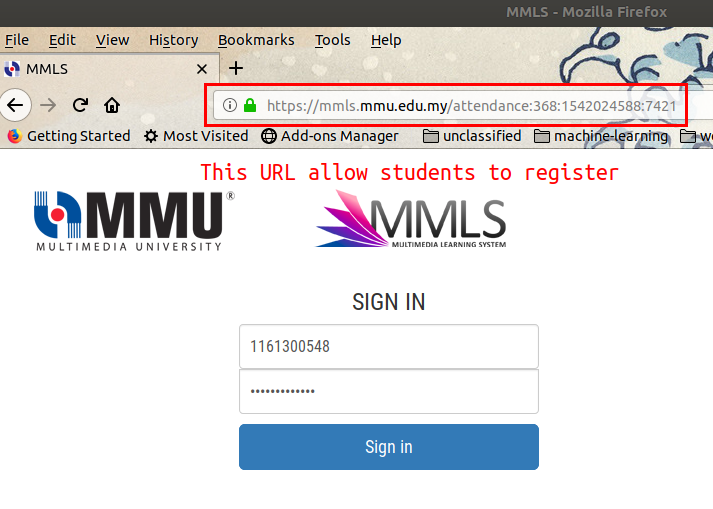
\includegraphics[width=\textwidth]{imgres/standard0_edit1.png}
\caption{HTML Page upon visiting the URL} 
\label{fig:std0}
\centering
\end{figure}

Referring to Fig. \ref{fig:std0} and Fig. \ref{fig:std1}, one critical aspect of the URL structure is that it follows a predictable format such that the final field of the URL is increasing, whereas the other 2 fields stay the same. \\
The two displayed URL :
\begin{center}
\url{https://mmls.mmu.edu.my/attendance:368:1542024588:7421}\\ 
\url{https://mmls.mmu.edu.my/attendance:368:1542024588:7776}\\   
\end{center}
are the same up until the final 4 digits, which is the final field. In fact, all MMLS registration URLs are the same up until the first colon ':' right after 'attendance'. Since there are no mechanism which the web server employs to track where a student gets their URL from, this means that the student can easily forge their own URLs given the predictable format of an increasing number at the final field. The challenge now is to guess the other 2 fields for other subjects as different subjects may have different fields. To achieve this, we compiled a list of URLs for different subjects and observed their pattern. The collected URLs are tabulated in Table \ref{tab:collectedurl} for comparison. As it was observed that the URL share the same structure, the table shall only highlight the differences in the URL.

\begin{figure}
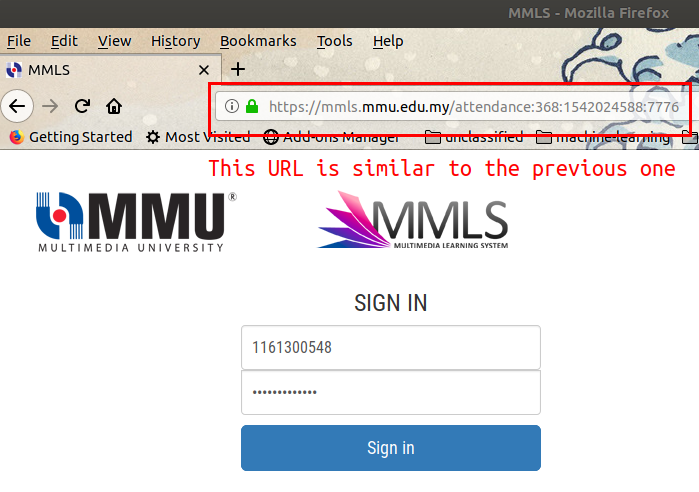
\includegraphics[width=\textwidth]{imgres/standard1_edit_painted.png}
\caption{Another URL} 
\label{fig:std1}
\centering
\end{figure}

If one is able to generate the URL correctly, this would break the dependency on friends as the attacker no longer need to wait for the URL to be sent to him or her in order to sign in attendance without being physically present. To expand further on this idea, the authors are interested to not only generate the URL for one subject, but for \textbf{all of the subjects} that the student is registered during the trimester. This is the first goal presented by this paper on the exploitation of the QR registration system on MMLS, named the \textbf{dependency goal}. Further sections of this paper shall denote the goal as \textbf{(DEP)}. 

This goal is an important one because if the attacker could not guess the correct URL, they will not be able to sign in their attendance for the class. They will then be required to either attend the class physically or request the URL from their friends should they desire attendance for any particular class.

\begin{table}
    \caption{Collected URL links from QR codes}
    \centering
    \begin{tabular}{|l|l|c|}
    \hline
    Subjects & URL & Timing (Start-End Y/M/D)\\
    \hline
    Security            & 368:1542024588:7421   & 17:00-18:00 2018/12/03\\
    and Cryptography    & 368:1542024588:8798   & 13:00-15:00 2018/12/05\\
                        & 368:1542024588:9352   & 13:00-14:00 2018/12/06\\
                        & 368:1542024588:10436  & 17:00-18:00 2018/12/10\\
                        & 368:1542024588:11878  & 13:00-15:00 2018/12/12\\
                        & 368:1542024588:12789  & 13:00-14:00 2018/12/13\\
                        & 368:1542024588:14407  & 17:00-18:00 2018/12/17\\
                        & 368:1542024588:15873  & 13:00-15:00 2018/12/12\\
                        & 368:1542024588:16121  & 13:00-14:00 2018/12/20\\
    \hline
    Advanced            & 1409:1541993846:6058  & 11:00-12:00 2018/11/29\\
    Microprocessors     & 1409:1541993846:7084  & 09:00-11:00 2018/12/03\\
                        & 1409:1541993846:9468   & 11:00-12:00 2018/12/06\\
                        & 1409:1541993846:10863  & 09:00-11:00 2018/12/10\\
                        & 1409:1541993846:12900  & 11:00-12:00 2018/12/13\\
                        & 1409:1541993846:14069  & 09:00-11:00 2018/12/17\\
                        & 1409:1541993846:16230  & 11:00-12:00 2018/12/20\\
    \hline
    Capstone Project    & 788:1541990282:6967   & 14:00-17:00 2018/12/03\\
    \hline
    Project Management  & 1865:1541992148:9191  & 17:00-18:00 2018/12/06\\
    \hline
    \end{tabular}
    \label{tab:collectedurl}
\end{table}

According to the list of collected URLs in Table \ref{tab:collectedurl}, one major observation is that the first and second field of a particular subject remains the same despite different classes. Attempting to link the class time to the numbers yield no relation, with the only pattern being observed is the linearly increasing final field with time. It is worthy to note that the total amount of digits for all 3 fields is roughly 16 (4+10+5) from the 1st, 2nd and 3rd field. The final column will increase by around 1000 after a day and around 3000 after a week. This observation shall be crucial in deducing an attack for the system later on. 

To achieve (DEP), one must find out how to generate the URLs for all the classes. Since the URLs are linked to the subjects tightly, a quick scan in the MMLS home page revealed that the numbers in the fields can easily be obtained from it as depicted in Fig \ref{fig:mmls0}. Using this method, the first and second fields of the registration URL link can be obtained from the home page. With this knowledge, the effective guessing space has dropped from \begin{equation}10^{16}\end{equation} to just \begin{equation}10^{5}\end{equation} on the 3rd field.

\clearpage{}

\begin{figure}
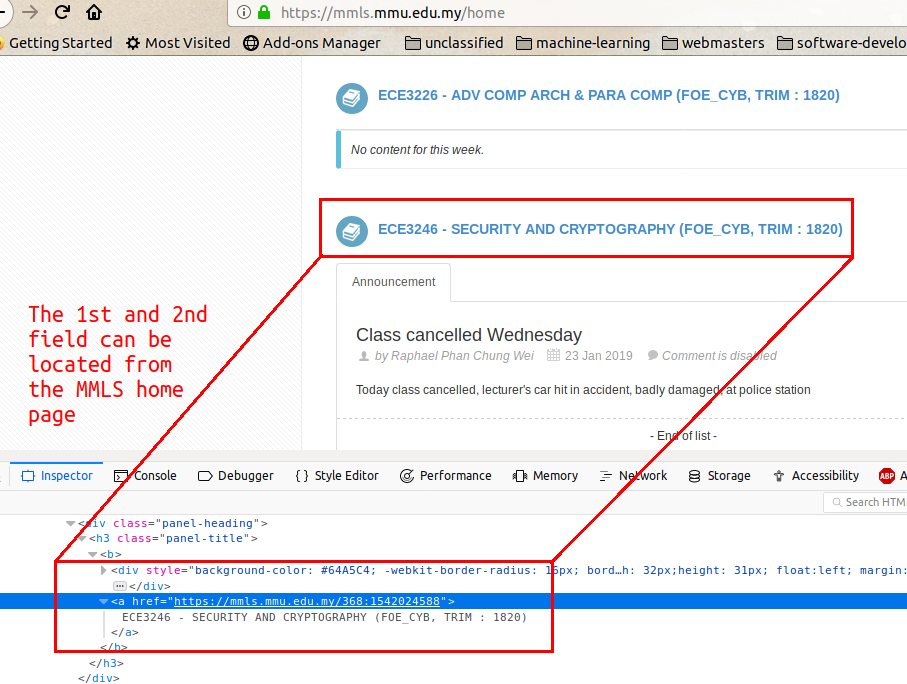
\includegraphics[width=\textwidth]{imgres/mmls0_edit_painted.png}
\caption{Retrieving the first and second field from the homepage}
\label{fig:mmls0}
\centering
\end{figure}

Thus, from the URL analysis, it can be concluded that the attendance URL has the following attributes: 
\begin{enumerate}
    \item 3rd field is increasing with time
    \item 1st and 2nd fields are linked to a particular subject
    \item 1st and 2nd field can be retrieved from the MMLS page
\end{enumerate}

\subsection{Registration Analysis}

From our analysis of the attendance URL, even if the student is able to generate their own URL, there is not much meaning when they have to wait until the class time to register successfully. The second goal of this paper now becomes clear, that is to allow the attacker to find out the possibility of registering attendance even if it is not within the period of the class. This goal comes with some integrity (INT) nature, as the attacker will be trying to submit a forged attendance registration to sign in outside the stipulated time. We call this goal the \textbf{timing goal}, denoted as \textbf{(TIM)}.

To understand more on the registration mechanism, a few registrations with different conditions were attempted with their behaviour noted down. The resulting behaviours were tabulated in Table \ref{tab:behaviour}. The Reply No. specifies an index for future references of a particular reply.

\begin{table}
    \caption{Registration result behaviour with different conditions}
    \centering
    \begin{tabular}{|l|l|c|}
    \hline
    Condition & Resulting behaviour & Reply No.\\
    \hline
    No previous registration record,     & The application replies with a message        & 1 \\
    student's first time registering    & "Your attendance has been successfully        &   \\
                                        &  updated."                                    &   \\
    \hline
    Previous registration record        & The application replies with a message        & 2 \\
    exists, student has already          & "Attendance already recorded for              &   \\
    registered before                   & this student ID."                             &   \\
    \hline
    Registering out of the class        & The application replies with an error         & 3 \\
    period (With or without             & "You are not allowed to check in as          &   \\
    previous record)                    & the current time is not the actual            &   \\
                                        & class duration.". See Fig. \ref{fig:den}      &   \\
    \hline
    Registering attendance for          & The application replies with a message        & 4 \\
    an invalid 3rd field number         & "You are not register to this class."         &   \\
    (Not any of the recorded            &                                               &   \\
    numbers)                            &                                               &   \\
    \hline
    \end{tabular}
    \label{tab:behaviour}
\end{table}

\begin{figure}
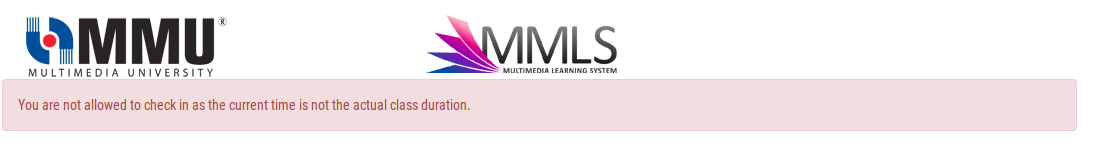
\includegraphics[width=\textwidth]{imgres/denied0.png}
\caption{Error when attempting to register past the class period} 
\label{fig:den}
\centering
\end{figure}

The URL is accessed and the form in which students submit in order to register attendance is observed and analyzed. Referring to Figure \ref{fig:reg0}, the form that was submitted upon clicking the "Sign In" button seems to contain some information regarding the period and date of the class. The fields were hidden but a simple element inspect on web browsers could let users access the form. A test was conducted to check if it is possible to launch a parameter tampering attack in which the date and time are changed and the form is sent back to the server. A simple method described below could then be used to verify if the attacker has succeeded based on the observations in Table \ref{tab:behaviour}.

\begin{enumerate}
    \item Obtain a valid URL and do not register for it.
    \item Once the class period is over, attempt to register.
    \item Expect Reply No. 3
    \item Edit the form using the web browser's developer tools
    \item Change the date to today's date
    \item Change the starting time to one hour before now.
    \item Change the ending time to one hour after now.
    \item Click Sign in again
    \item Observe Reply No. X
\end{enumerate}

\clearpage{}

If X was 1, we theorize there are two outcomes which could cause this scenario. The first one being that the client side mistakenly thought that the student has registered within time and has created the reply. However, in this case, the server may not have registered the attendance as it contains it's own validation mechanism. We know that scenario 1 is unlikely as closer inspection on the HTML source found no traces of validation on it's Javascript content. The other scenario being that the server has successfully received the students request and has registered the student into the attendance list for that particular class.

Nevertheless, to truly ensure that the server has indeed registered the attendance of a student after tampering with the parameters on the form, one could run the steps again from step 1 using the same URL. Except this time instead of receiving Reply No. 1, they would receive Reply No. 2.

Upon receiving Reply No. 2, the students now know that they have indeed registered for the attendance. (TIM) is achieved because the only way for the server to reply this message is when it has a previous record of the student registering the attendance for that particular class. The client will not store the student's registration history.

\begin{figure}
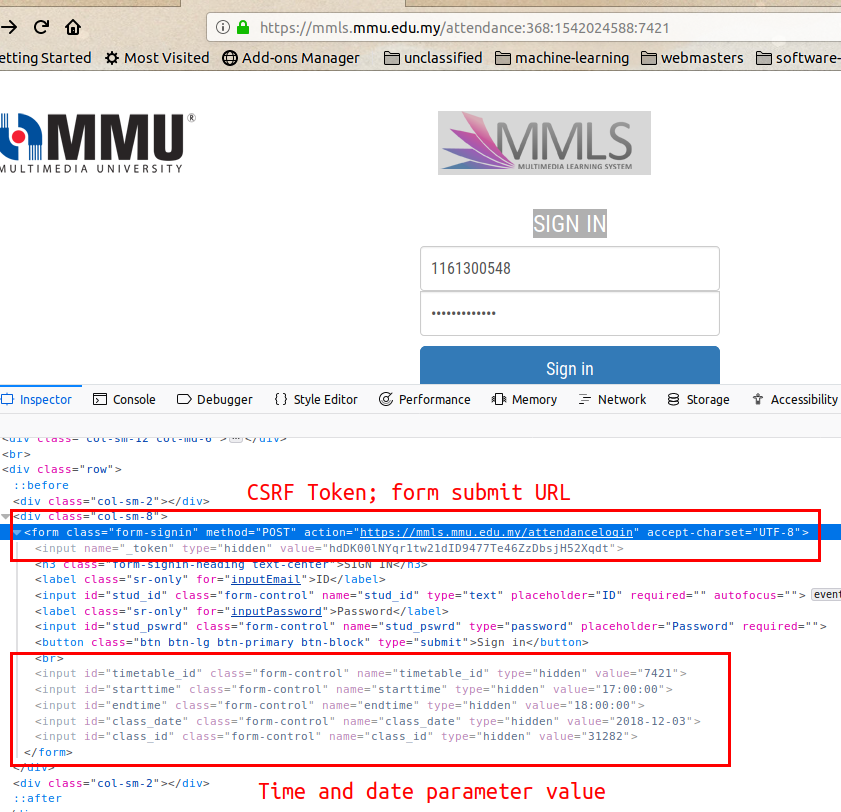
\includegraphics[width=\textwidth]{imgres/reg0_edit.png}
\caption{Date and Time parameters on the HTML form} 
\label{fig:reg0}
\centering
\end{figure}

The form as depicted in Fig. \ref{fig:reg0} also shows a CSRF token embedded with it. Upon checking the network packets sent out during the loading of the registration page, The use of session cookies is also noted. As the users who employ our proposed method of attack are most likely malicious users, or misbehaving students, this meant that the CSRF token and session cookie is of no security concern to us as there is no cross site requests or session hijacking. Since the students themselves are requesting for the forms from the MMLS attendance registration page, the CSRF and session cookie are naturally given to them.
% TODO: analysis on the stime - etime parameter tampering vuln.
% TODO: introduce the second goal of paper, the TIMING GOAL (TIM)
% TODO: analysis on the token / session ID

\clearpage{}

\section{Attack methodology}
% TODO: the methods we come up with
% TODO: how feasible is it
\newcommand{\theattack}[1]{\textit{the attack}}
\newcommand{\scanattack}[1]{\textit{scan attack}}

With the conclusions obtained from the analysis, it can be concluded that it is \textbf{possible} for a student to register for a particular class even if they have missed the class' period and has no friends to send them the URL. We shall call this attendance registration which comprises of the basic guess of the attendance URL and change of timing parameters, \theattack{}. Hence, the question of how feasible is \theattack{} arises. 

\subsection{Feasibility}
Currently, the 3rd field can only be obtained through guessing. What is the maximum number it can reach up to? From our observations in Table \ref{tab:collectedurl}, a week will knock up about 3000 for the number. A long trimester in Multimedia University which attendances are taken and counted consists of 14 weeks, while a short one is 7 weeks. This meant that the maximum number that the 3rd field will go up to is approximately \noindent\begin{equation}
    14 * 3000  = 42000 
\end{equation} However, we shall consider a full 5 digit number space, giving us a number space of \noindent\begin{equation}10^5 = 100,000 (0-99,999)\end{equation}    
The attacker will have to first guess the 3rd field parameter correctly (DEP). Although there is some reference on time, this still requires a huge effort as the attacker will have to go through the hassle of inputting or modifying the 3rd field of the URL link of a specific class \textbf{one by one} manually. After guessing, they will then need to register for that class by tampering the time parameter on the form to achieve (TIM). In short, \theattack{} is hard to execute because of the uncertainty in the 3rd field of the registration URL and the tedious need for users who want to register for more than one class to do the modification which requires some precision and time.

With such attacking scheme, the effort of the attacker in trying to achieve (DEP) and (TIM) would be a lot greater than the gain obtained from performing \theattack{}. This would defeat the purpose of \theattack{} as it would be much easier for them to just attend class or request for an URL and register during class time instead. We say that \theattack{} only achieves (TIM) but not (DEP) feasibility wise as students will still require a valid URL sent to them from their friends who actually attended class.

\subsection{Scanning Attack}

Despite the in-feasibility of \theattack{}, it is still a usable method to sign for attendance. What if one could automate the process of guessing and tampering, performing an attack similar to brute-force guessing of passwords, but on URLs instead? If that can be achieved, \theattack{} can be transformed into a \scanattack{}, in which the number space of the 3rd field is exhausted to obtain all the possible URLs. The results is then saved for the users to see and to verify their attendance, if they want. In order to know if a particular class URL exists, one would expect Reply No. 1 or 2 from Table \ref{tab:behaviour} upon tampering with the date and time parameter. This means that a Reply No. 4 on a URL will imply that it is an invalid URL. A \scanattack{} is simply an automated barrage of \theattack{}. A simple flowchart on Fig. \ref{fig:flowchart_scan} demonstrates the sequence of the \scanattack{}.

\begin{figure}
    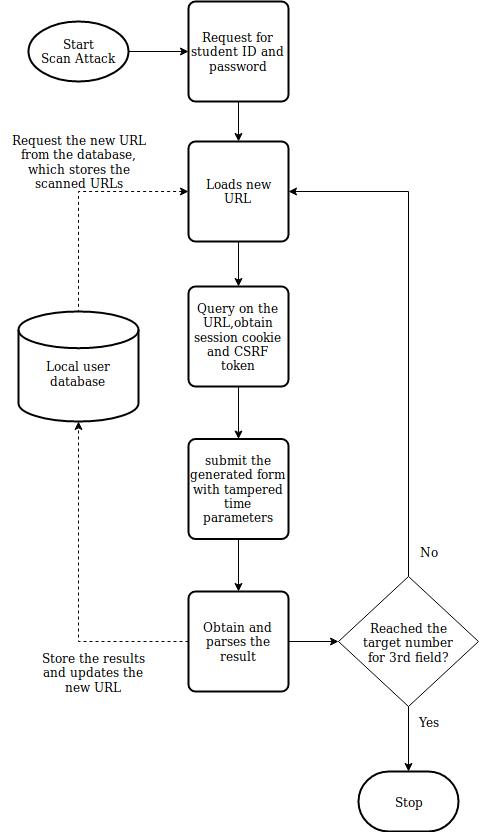
\includegraphics[width=0.87\textwidth]{imgres/flowchart_sleepin.png}
\caption{Flowchart for the \scanattack{}} 
\label{fig:flowchart_scan}
\centering
\end{figure}

We designed and developed a command line interface computer Java program, which we named \textbf{Sleepin}, to perform the \scanattack{}. This program carries out the flow as depicted in Fig. \ref{fig:flowchart_scan}
in a controlled manner, tremendously reducing the effort to gain ratio which has tied down \theattack{}. 

\subsubsection{Sleepin:}
Firstly, Sleepin will attempt to log in to MMLS with the attacker's student ID and password. As MMLS is intended only for web browsers' access, A HTTP client is launched in the background to retrieve the CSRF token and session cookie from the web browser which will then be used later in order to fool the MMLS server into thinking that the program that is trying to log in to it is a web browser. To further mimic the traffic between the web browser and the MMLS server, using developer tools on a modern browsers, the packets that are sent via a POST request are thoroughly analyzed to allow Sleepin to produce a very similar request to that of a browser. Referring to Fig. \ref{fig:header_analysis}, the cookies as well as the form parameters are analyzed to allow us to forge a very similar request structure to that of a web browser.  

\begin{figure}
    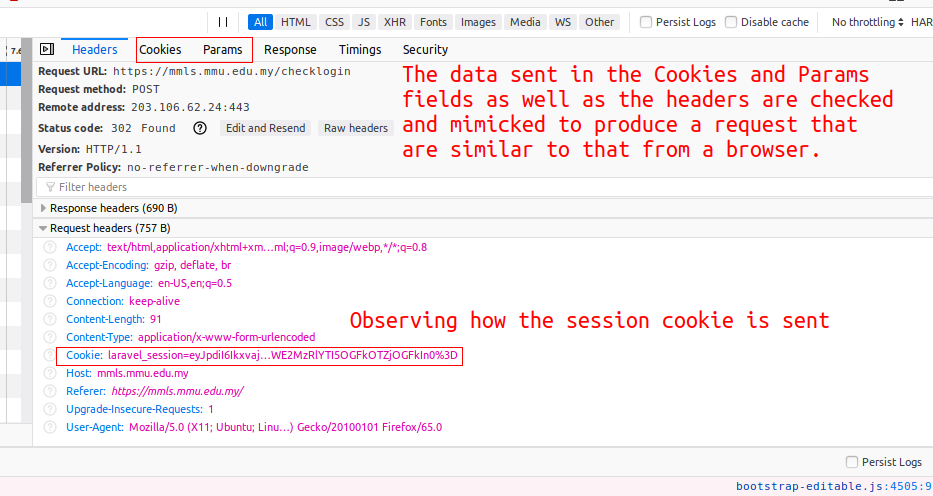
\includegraphics[width=\textwidth]{imgres/header_analysis.png}
\caption{Network packets from a login request to the MMLS server} 
\label{fig:header_analysis}
\centering
\end{figure}

Once the attacker has successfully logged in to MMLS, the program will retrieve all the subjects which the user is registered with MMLS for the current trimester from the MMLS server and display it in a list. This process retrieves all of the subjects' 1st and 2nd fields in the registration URL structure. From there, the attacker can perform several actions which are related to the \scanattack{}:
\begin{itemize}
    \item perform \theattack{} on a specific subject in the list for a specific number of instances. This is the \scanattack{}.
    \item re-range or change the starting and ending values of 3rd field used for URL generation by the \scanattack{}.
    \item perform \theattack{} on a specific 3rd field number.
    \item specify the current scan value (3rd field of URL) of a specific subject.
    \item display the result of \scanattack{} of a specific subject
    \item output the result of \scanattack{} of a specific subject in a .csv file.
    \item permanently delete all results of \scanattack{} of a specific subject.
\end{itemize}

\clearpage

If a \scanattack{} is to be launched by the attacker, the URL link(s) will be generated accordingly, depending on the subject selected as well as the number of instances and/ or the starting and ending values of the 3rd field of the URL links specified. For each 3rd field value, once the corresponding URL link is generated, it is queried onto the MMLS server, retrieving the correct session cookie and CSRF token. Sleepin will then forge an attendance form with the stored CSRF and time parameters changed to allow the attacker to log in at current time. Specifically, the class time will be changed to:
\begin{center}
    start time  : current time - 1 hour\\
    end time    : current time + 1 hour\\ 
\end{center}

Then, the form will be submitted to the MMLS server along with the relevant headers and the stored session cookie as an attempt to register the attendance. The reply obtained from this sequence will be stored in a local database to allow the attacker to view and analyze at a later time. Since the local database is updated every time \theattack{} is launched by the \scanattack{}, this meant that the program can be terminated at any time and be resumed later on to continue the \scanattack{}.

\section{Implementation and Result}
% TODO: the app showcase (sleep-in)
% TODO: proof of success
With the development of Sleepin, it is said that the effort required for the attacker to register attendance will be reduced significantly. In this section, we will show the results of the implementation of the proposed solution.

Upon launching Sleepin, the interface as shown in Fig \ref{fig:sleepin_login} will be shown, requesting attacker to log in to MMLS. Note that the attacker is advised not to perform a \scanattack{} after 11pm as the class' end time will be modified as per below. This will cause the class' end time to be on the next day (having a different date),  which may possibly cause the attendance to not be registered correctly. The modification is done so that the attack achieves (TIM).
\begin{center}
    end time = current time + 1 hour\\
\end{center}

\begin{figure}
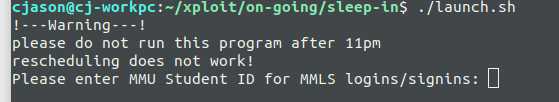
\includegraphics[width=\textwidth]{imgres/sleepin_login.png}
\caption{Interface of Sleepin for attacker to log in to MMLS} 
\label{fig:sleepin_login}
\end{figure}

Once the attacker has successfully logged into his/ her own MMLS account, the subjects which the attacker is registered on the current trimester will be displayed with each subject having its own selector ID, as shown in Fig \ref{fig:sleepin_show}. The selector IDs are for the attacker to specify which subject's class' attendance to register. As highlighted in Fig. \ref{fig:sleepin_show}, the start and end values of a \scanattack{} on each subject, indicating the first and last values of the 3rd field parameter in the attendance URL on which \scanattack{} can be performed for each subject, and the current scan value of each subject, indicating the highest scanned value for the 3rd field parameter in the attendance URL of a particular subject, are also shown to the attacker. This list of subjects can also be viewed by the attacker by inputting "show" when Sleepin requests for input. 

\begin{figure}
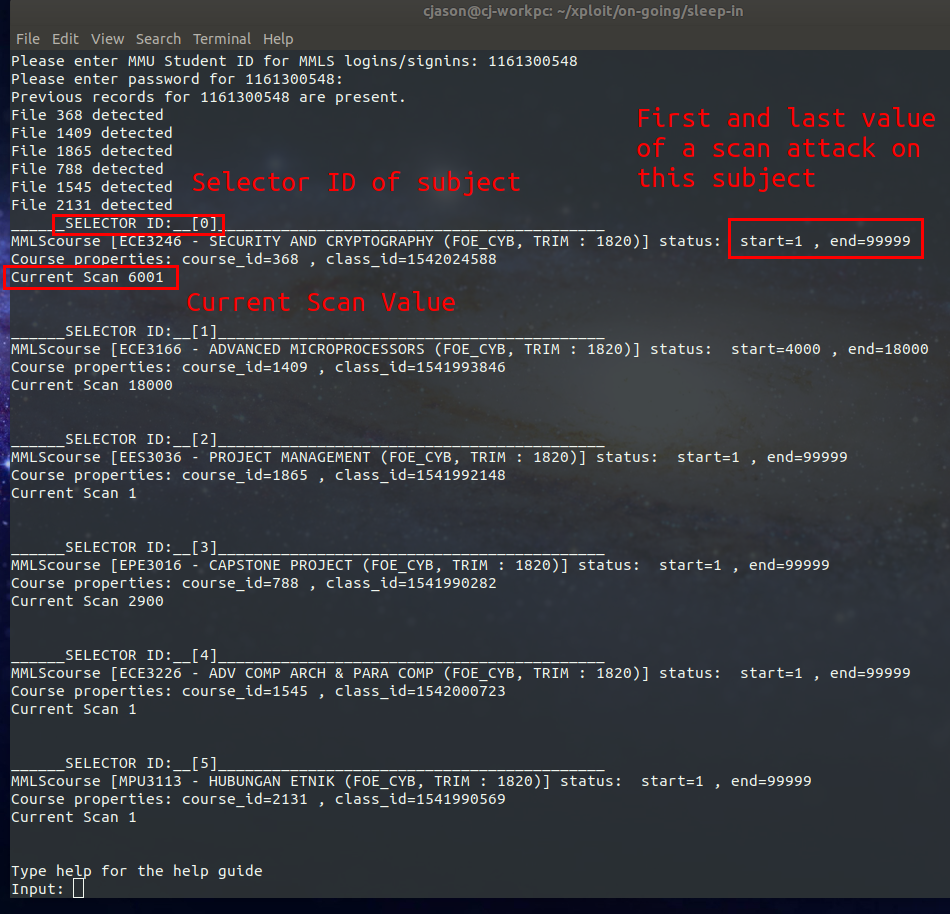
\includegraphics[width=\textwidth]{imgres/sleepin_show.png}
\caption{List of registered subjects and their selector IDs} 
\label{fig:sleepin_show}
\end{figure}

From here onwards, the attacker can choose to perform several different actions. Inputting "help" will display the help screen as shown in Fig. \ref{fig:sleepin_help} to allow the attacker to know what actions can be performed using this program and how to perform them.

\begin{figure}
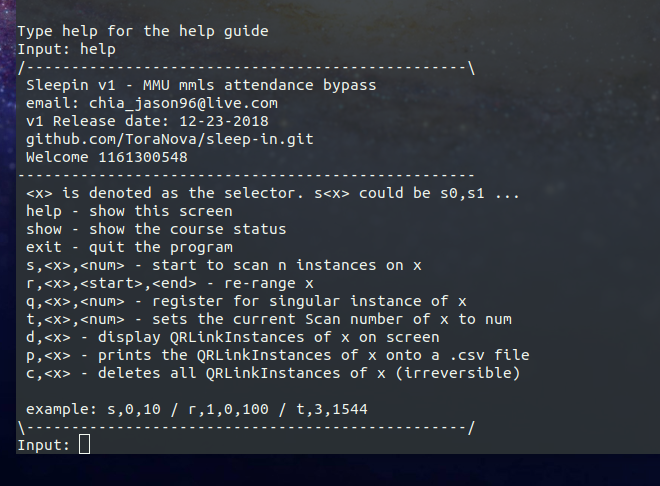
\includegraphics[width=\textwidth]{imgres/sleepin_help.png}
\caption{Sleepin help screen} 
\label{fig:sleepin_help}
\end{figure}

If the attacker knows a specific 3rd field parameter of an attendance URL for a specific subject's class, \scanattack{} can be performed on the identified 3rd field parameter value as shown in Fig. \ref{fig:sleepin_single_instance}. This can be used to test a particular 3rd field parameter of an attendance URL to test the hypothesis of the attacker, if not to sign in attendance of a specific class which the 3rd field parameter is already known to the attacker, either to confirm the registered attendance to obtain Reply No. 2, to register attendance to obtain Reply No. 1 in order to test whether Sleepin can perform its intended purpose during the testing stage, or to register attendance when the 3rd field parameter is obtained from the attacker's friend. 

\begin{figure}
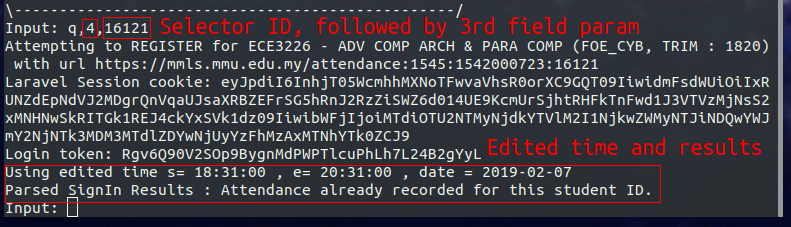
\includegraphics[width=\textwidth]{imgres/sleepin_single_instance.png}
\caption{A \scanattack{} of one cycle being performed on a single 3rd field parameter} 
\label{fig:sleepin_single_instance}
\end{figure}

Other than that, the attacker can update the current scan value of a particular subject if a \scanattack{} is to be performed from a specific 3rd field parameter value, which the previous \scanattack{} had yet to achieve or had exceeded, as depicted in Fig. \ref{fig:sleepin_update_scan_value}. 

\begin{figure}
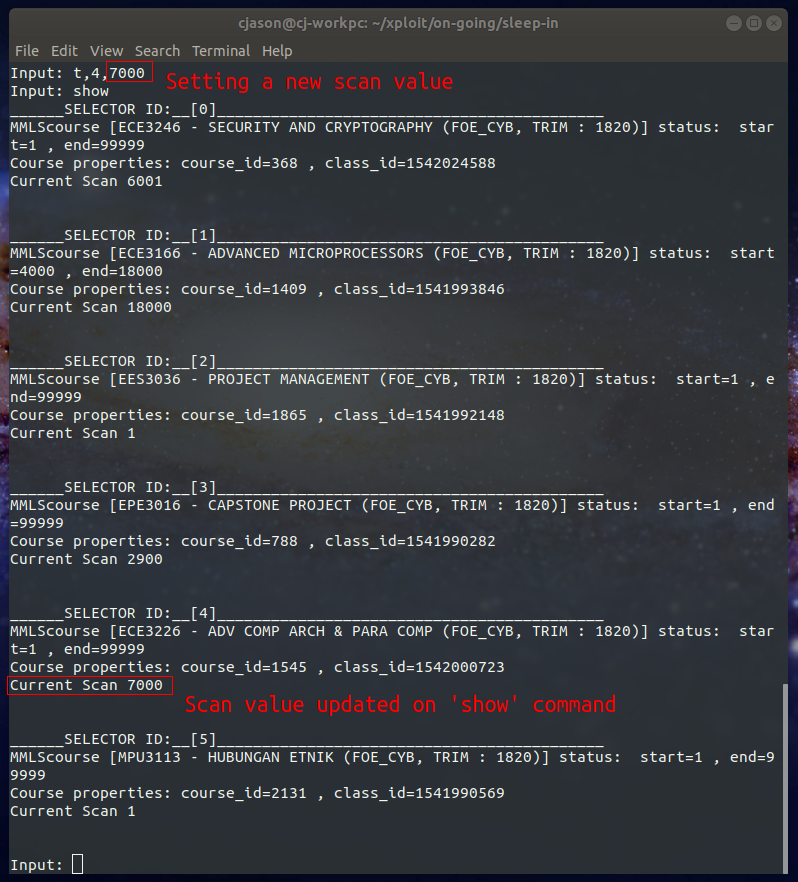
\includegraphics[width=\textwidth]{imgres/sleepin_update_scanval.png}
\caption{Update the current scan value of a particular subject} 
\label{fig:sleepin_update_scan_value}
\end{figure}

A specific number of cycles for a \scanattack{} can be performed on a selected subject, starting from the attendance URL with the 3rd field parameter being the current scan value of that subject. For instance, Fig. \ref{fig:sleepin_scan_for_x} shows the action of a scan attack of 1000 cycles performed on the subject with the selector ID of 4, starting from the current scan value of 1. This method allows the \scanattack{} to break (DEP).

\begin{figure}
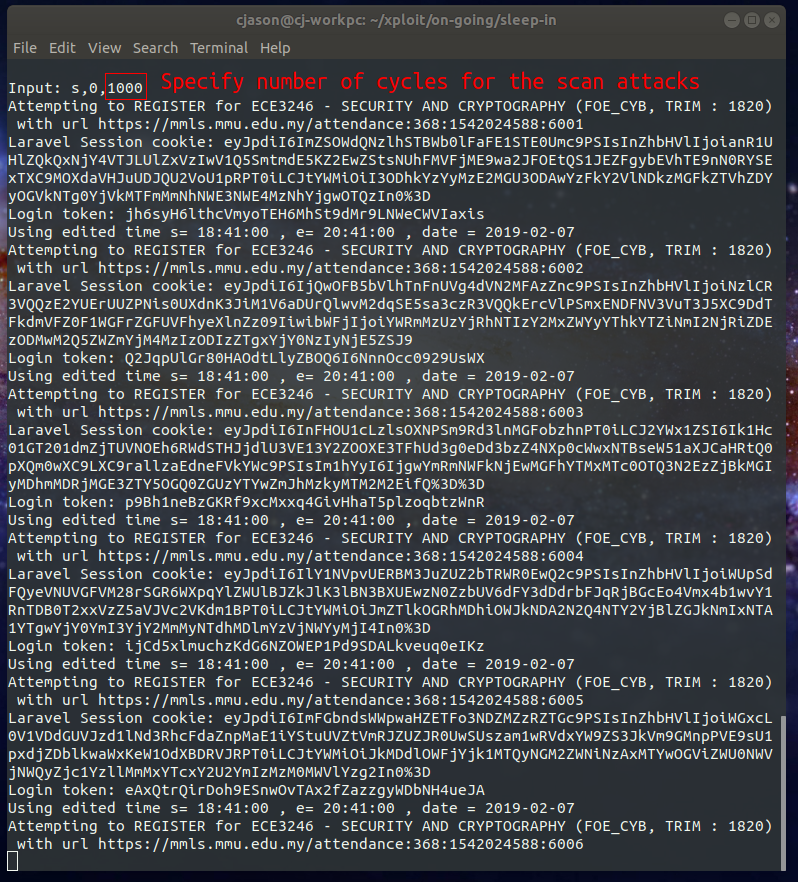
\includegraphics[width=\textwidth]{imgres/sleepin_scanx.png}
\caption{Perform \scanattack{} on a particular subject for a specified number of instances/ cycles} 
\label{fig:sleepin_scan_for_x}
\end{figure}

Once a \scanattack{} had been performed, its results can be displayed on screen, as shown in Fig. \ref{fig:sleepin_display}, for the attacker to see, observe and analyze. Additionally, the results of a \scanattack{} can even be outputted in a .csv file as shown in Fig. \ref{fig:sleepin_csv_result}, using a command as depicted in Fig. \ref{fig:sleepin_csv}. This is to ease the attacker to perform analysis as the results can be filtered to read the pattern more easily using the built-in functions of .csv file.  

\begin{figure}
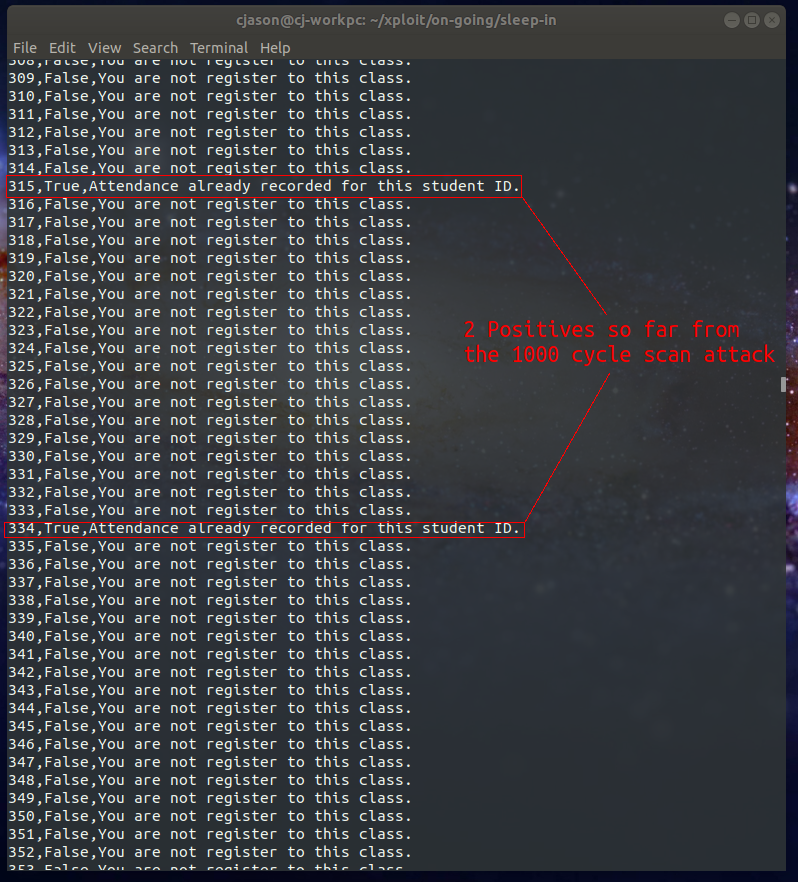
\includegraphics[width=\textwidth]{imgres/sleepin_display.png}
\caption{Results of \scanattack{} displayed on screen} 
\label{fig:sleepin_display}
\end{figure}

\begin{figure}
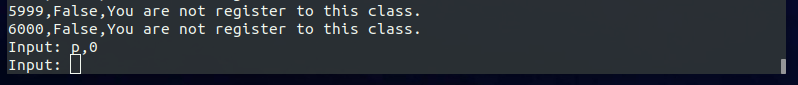
\includegraphics[width=\textwidth]{imgres/sleepin_csv.png}
\caption{Command to print results of \scanattack{} in a .csv file} 
\label{fig:sleepin_csv}
\end{figure}

\begin{figure}
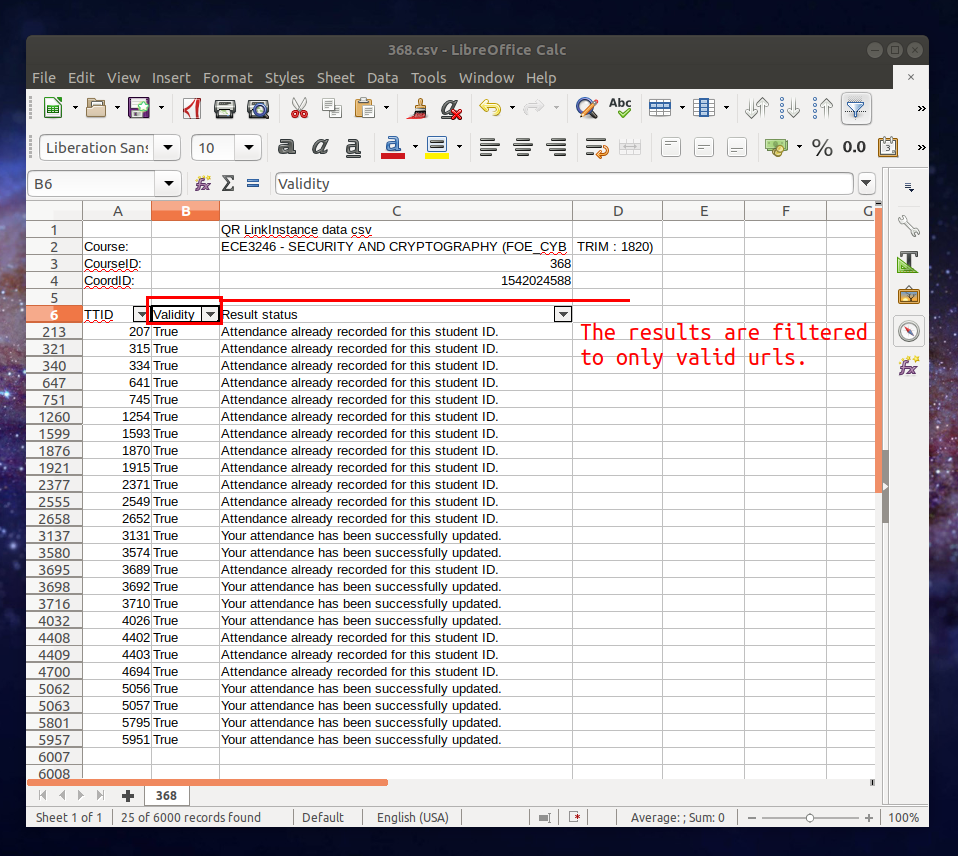
\includegraphics[width=\textwidth]{imgres/sleepin_csv_output.png}
\caption{Filtered results of a \scanattack{} outputted in a .csv file} 
\label{fig:sleepin_csv_result}
\end{figure}

In order to confirm the registered attendance, the attacker can either re-do or perform the \scanattack{} on the same range of 3rd field parameters of attendance URL and expect Reply No. 2 for all the valid 3rd field parameter values, or check their subjects' attendance percentage in their MMU CaMSys accounts and expect an increase in percentage of attendance. Thus, the attacker can confirm whether the attendances have been registered successfully on his/ her own without having to hack into another system or go through the lecturer of subject coordinator of the given subject. 

Furthermore, the range of 3rd field parameter values of attendance URLs of a particular subject to be scanned using a \scanattack{} can be changed according to the needs of the attacker as shown in Fig. \ref{fig:sleepin_rerange}. Therefore, no worries about the 3rd field parameter of the attendance URL growing beyond the default maximum value. It can be adjusted accordingly. In extension to that, the current scan value of the selected subject will change to the 3rd field parameter value in the first cycle of a \scanattack{} of a subject if the original current scan value is out of range. 

\begin{figure}
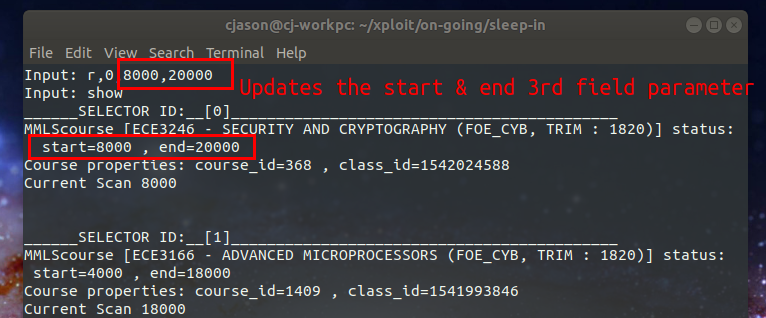
\includegraphics[width=\textwidth]{imgres/sleepin_rerange.png}
\caption{The range of a \scanattack{} cycle on a particular subject is updated} 
\label{fig:sleepin_rerange}
\end{figure}

As a proof of ease of \scanattack{} by the attacker, the period of time required for the attacker to perform a \scanattack{} of size 1000 on a few devices are recorded in Table \ref{tab:timetaken}. This is due to the fact that the \scanattack{} speed depends on the internet connection speed as well as the device's processing speed.

\begin{table}
    \caption{Time taken for different devices to complete 1000 cycles of the \scanattack{}}
    \centering
    \begin{tabular}{|l|c|}
    \hline
    Device       & Time Taken / 1000 Cycles (seconds)\\
    \hline
    1            & 536\\
    \hline
    2            & 446\\
    \hline
    3            & 483\\
    \hline
    \end{tabular}
    \label{tab:timetaken}
\end{table}

Therefore, the average time taken to complete a \scanattack{} of 1000 cycles would be:
\begin{equation}(536 + 446 + 483)/ 3 = 488.33s \approx 8min:8s\footnote{s - seconds, min - minutes, hr - hours} \end{equation}

Thus, the average time taken to complete \textbf{ONE} cycle of a \scanattack{} would be:
\begin{equation}488.33/ 1000 = 0.488s\end{equation}

Theoretically, from the observation of the currently gathered data, each subject's \scanattack{} ranges from the 3rd field parameter value of 1 to 99999, taking up 100,000 values. Thus, a full range \scanattack{} (100,000 cycles) performed to register a 100\% attendance for a single subject will consume approximately:
\begin{equation}0.488* 100,000 = 48,800s \approx 813 min:20s \\\approx 13 hr:33 min \end{equation}

In each trimester, a MMU student can register up to 6 subjects, in maximum. Continuing from the previous theoretical calculation, the total time taken for the attacker to perform \scanattack{}s to register attendance for all 6 subjects would be approximately:
\begin{equation}14 hours * 6 = 84 hr  \approx  3.5 days  \approx  3 days : 12 hr\end{equation}

Just by running Sleepin for around 4 days continuously, the attacker can be marked as "present" for all registered subjects' classes without having to attend any of the classes physically. Hence, it is proved that by performing \scanattack{}s using Sleepin, (TIM) and (DEP) can be achieved very easily. The effort of performing \scanattack{} to the gain of having marked present in all classes is greatly skewed, making it very attractive for students to use the method rather than attending class itself. 

\subsection{Unexpected Observations}
Upon going through a list of a \scanattack{} that has a 3rd field parameter of 1 until a value slightly above the theoretical limit of a trimester, an interesting observation is noted such that the number of valid URLs far exceed the number of actual classes in the given trimester. Referring to Fig. \ref{fig:sleepin_obs}, notice that out of 47723 cycles, 137 of them return as a valid URL. Suppose that a subject will have 3 classes during a week, the total amount of classes in a semester should not exceed 3*14 = 42 classes. This meant that the amount of valid URLs should also be less than that of 42.

\begin{figure}
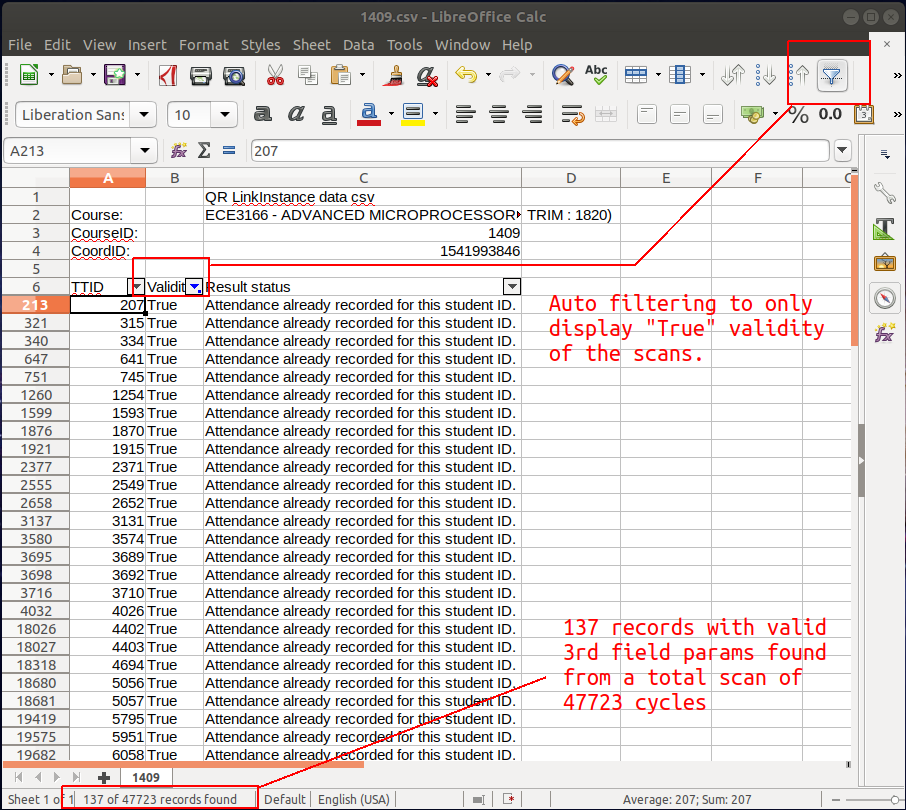
\includegraphics[width=\textwidth]{imgres/sleepin_observation.png}
\caption{Anomaly detected by a full cycle \scanattack{}} 
\label{fig:sleepin_obs}
\end{figure}

However, our results show that the number of valid URLs far exceed that of our expectation by roughly 3 times that amount. We theorize that there are a few possible explanations for this phenomenon, that is

\begin{enumerate}
    \item Different sections of the same subjects have the same 1st and 2nd field parameters. Hence, the lecturers will have to generate at least 3 times as much URLs if there are 3 different sections considering both lecture classes and tutorials. This scenario assumes that lecturers generate the QR code as needed.
    \item The system pre-generates all QR codes and assigns them to a lecturer \\throughout the semester, and it is designed to generate extra QR codes so that it can never run out of them.
    \item Since there are 3 lecturers in charge of the subject from our observation, perhaps the amount of URLs vary proportionally to the amount of lecturers teaching a subject.
\end{enumerate}

The first explanation becomes impossible by a simple experiment. An attempt to register for a friend's class that is of another section on the same subject results in a Reply No. 4, which meant that students must only register attendance onto their own respective sections only.

The third explanation also becomes unlikely upon performing a \scanattack{} on a subject taught by only one lecturer. From the results of the \scanattack{} as shown in Fig. \ref{fig:sleepin_obs2}
, it is revealed that the number of valid URLs exceed the expected number by almost the same ratio. Therefore, this explanation is not suitable to be treated as the true reasoning behind the phenomenon.

There is not enough information for us to analyze and make a deduction on the second explanation. However, currently, it best suits to be the explanation of the observation discussed in this section. 

\begin{figure}
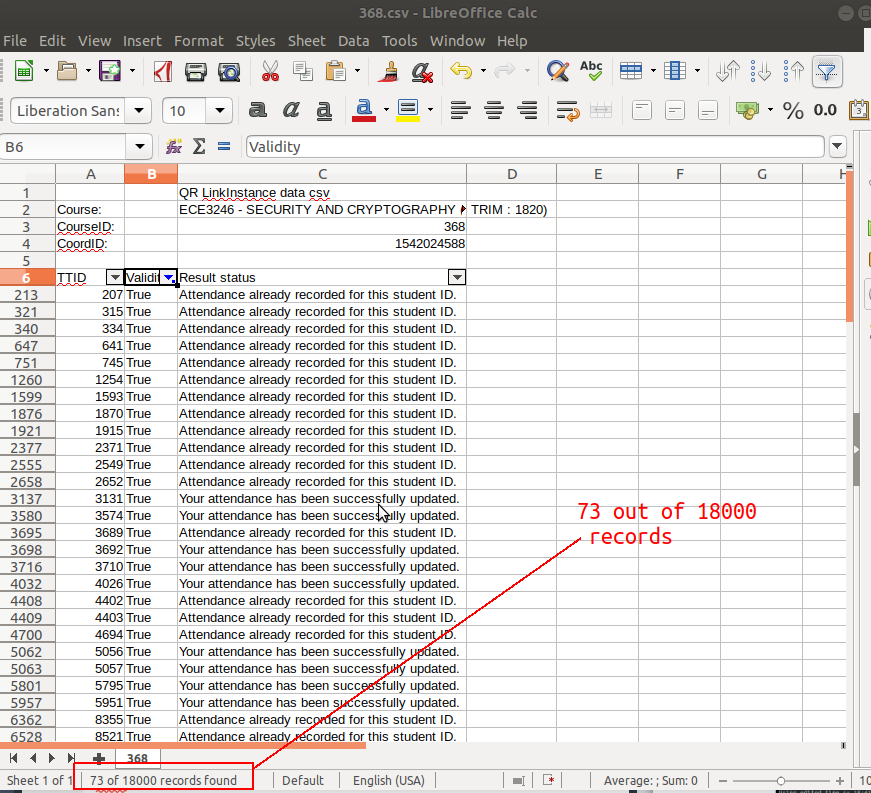
\includegraphics[width=\textwidth]{imgres/sleepin_obs2.png}
\caption{Results from a subject with only 1 lecturer} 
\label{fig:sleepin_obs2}
\end{figure}

\section{Suggestions for mitigation}
%TODO : Write about the suggestions on how to mitigate
Here, we introduce a few ways so that the MMLS attendance system is able to be upgraded to defend itself against both \theattack{} and the \scanattack{}. We shall discuss the suggestions in relation to the goals proposed in this paper, namely the timing goal (TIM) and the dependency goal (DEP). 

\subsection{Suggestions to strengthen (DEP)}
Let us first remind ourselves what does it mean when an attacker achieves (DEP)? An attacker is said to achieve (DEP) if they are able to reliably generate the correct URL that allows them to sign in their attendance without obtaining it from their friends or from the QR code projected on the screen. We see that \theattack{} is unable to break this goal as the effort needed to reliably generate the URL is far greater than actually attending the class and scanning the QR code projected on the screen or requesting a friend to send the URL. However, the \scanattack{} is able to break (DEP) with ease due to it's predictable nature. With this, we present our first suggestion.

To ensure (DEP) is not broken by a \scanattack{}, the system will need to make sure that it does not generate the URL in a linearly increasing/ decreasing fashion or any other predictable patterns, but rather randomly generating them like how one would generate CSRF tokens. 

Suppose a number space from 0-9, whereby we will have 2 types of system. The first system generates the number in an increasing fashion, that is, 0,1,2,3 ... 9. This system is analogous to the current MMLS system. The second system generates the number randomly and does not have a predictable sequence. For the first system, the more numbers that were generated, the lesser the number of guesses required by the attacker. For instance, an attacker who found out that 4 is the last valid URL would be certain that 0,1,2 and 3 are already generated and will not consider their possibilities in future guesses. However, for a system that generates the number randomly, an attacker armed with the knowledge that 8 is the latest generated number will still have to guess every single number in the number space except 8. This meant that the guessing space remains constant even if numbers are being generated.

If the attendance system generates the URL in a random fashion, this tremendously powers up the system in terms of (DEP), as the attacker will require a greater amount of effort to guess the right URL to register. This is because in order to guess even just one URL, the attacker will need to start from 1 and end at 99,999. This difficulty remains the same for the second, third and all future URLs. For the previous scheme, the attacker just have to start from where they stopped and hit the next valid URL to allow them to register. However, this is not enough as the attacker may simply choose to perform the attack near the end of the trimester when all the URLs are already generated. Thus, alphabet characters in both upper case and lower case should also be used to represent the 3rd field parameter to significantly buff up the difficulty in guessing. This will increase the guessing space from 100,000 to 62 \textsuperscript{5}, which surmounts to a whopping 916,132,832 possibilities. If each URL takes 0.488 seconds, this meant the total time it takes to exhaust all the possibilities will be about 5,174 days or 14 years. This will ensure that the student is unable to exhaust the space even in the span of their undergraduate studies, thus demotivating them from using the  \scanattack{}s to register for their attendances.

Another simple suggestion to strengthen the system against a \scanattack{} without changing the structure of the URL would be to limit the number of sign-ins to the attendance server by the students on a daily basis. If the system only allows a maximum of 10 attendance registrations per day, then an attacker would not be able to effectively carry out the \scanattack{}.

\subsection{Suggestions to strengthen (TIM)}
We say an attacker has broken (TIM) if they are able to register their attendance even when the class time is over. This is currently possible because the attendance registration form that was sent from the registration site contains the date and time parameters of a particular class. This can easily be secured by introducing server-side sanitation that detects or prevents parameter tampering. For example, before sending out the form for a student to fill in and register their attendance, the server could run a hash function on critical information such as class period and date and store the digest for that particular session. Upon the submission of the form by the student, what the server has to do is to compute the hash of the critical data in the submitted form again and re-check with the stored digest to see if the important parameters are tampered with. This problem behaves similarly like the Integrity problem (INT), where the server must have it's own mechanism to verify whether a form's parameters that are not intended to be edited has been tampered with.

A cleaner solution to this problem is to not send the date and time parameters on the form. The server should instead look-up on a stored database of classes and compare it with the server's local time to ensure that a student is registering within the class' duration. This totally annihilates the possibility of parameter tampering as there are no parameters to tamper with. With this, the attacker will not be able to achieve (TIM) as the server now runs a strict check using it's own database and it's own clock.

\subsection{Additional Suggestions}
Other than methods to strengthen against (TIM) and (DEP), this section discusses the additional measures that could serve the system well in its defense against malicious students aiming to bypass the integrity of the University's attendance record. 

Primarily, the geo-location information of a student attempting to sign in should be taken into consideration. The system should ensure that the registration comes from within the university by retrieving the location of a student attempting to sign in. This could be feasible since registration by students are done using their phones, and modern phones are built in with global positioning systems that allows their geographical information to be sent. This ensures that a person registering an attendance is at very least in the premise of the university. 

A simpler solution exists if the university wants to ensure that a student is actually within university premise when they register their attendance, that is to only accept registration within the university network. A student must first connect to the university's wireless network first before attempting to register their attendance, this ensures their presences in the university premise as their registration originates from within the network. As the wireless signal decreases exponentially with distance, an attacker that is at home will not be able to register as they will not be able to connect to the university's network.

However, the above methods assumes that an attacker intends to register even at the comfort of their homes. However, some attackers may be skipping class in university premise or are staying in the hostel or dormitory situated within the university premise, which makes it difficult to distinguish if a student is really within a class during the stipulated time. For instance, a student could be absent for a class while still within the University, and upon receiving a QR code sent to them by their friends or by using the methods proposed in this paper, they are still able to register their attendance despite not being physically in class as location based tracking is only able to pinpoint a student's location down to a few hundred meters, which allows them to be outside of a class and still be within the general vicinity of it. A suggestion to overcome this problem is to use a custom smart phone application that does the scanning of the QR code rather than a generic QR scanner. The application should snap a picture of the student and the surrounding using the phone's front camera while scanning the QR using the phone's main camera. This allows a lecturer to verify if a student is indeed in class or not during the registration of their attendance via QR code should suspicion arises.

\section{Analysis and Discussion}
This section provides some analysis on attendance systems and a discussion about their drawbacks.

\subsection{Rationale on a QR attendance systems}
\textbf{A means of authenticating a person at a specific location within a specific time is key to have a solid registration system}. If we take a look at conventional paper and sign method, it only achieves validity in terms of time and location, as the signature sheet is only available during class time and at the class location. there exist an authentication (AUTH) problem since a signature can be faked by a friend. A lecturer wants to know if an attendance is truly generated by the student themselves. They can never be able to truly tell apart if a signature is masterfully forged by another student. Even if he/ she can, the issue will become debatable as human signatures may vary from time to time. 

A URL-based QR registration system in its naked form comprises of registration URLs encoded in the QR code. This causes it to lack as a registration system because the links could be shared easily and \textbf{remotely}. Although it achieves (AUTH) in the sense that only the student themselves will have access to their own student ID and password combination, it is lacking in terms of validity in time and location. MMU's QR attendance system failed in terms of timing validity as (TIM) is broken by a parameter tampering attack. The timing validity can be solved by implementing server side checks on the time, but the notion of validating a student's location when they register their attendance is a difficult one even with pictures as the lecturer's may need to go through the list of registration and examine the pictures one at a time. With geo-location recording, on the other hand, a student is still able to register outside of a class as long as they are within a few hundred meters in the vicinity of the class.

Thus, it is very difficult for a URL-based QR attendance registration system to have a solid and true attendance record as it inherently works with \textbf{remotely} accessible URLs. A more superior form of it is a QR based attendance paired with a trusted android application which does not works with URLs. An example of such a system is that an Android application which scans for a QR code that comprises of a random string generated by the server, and sends the string to the server using a socket connection that cannot be easily mimicked by other applications. The server then verifies the string and authenticate the registration of the student if it is within a specific time. If the application is designed in such a way that even if the user knows about the random string, they are unable to easily send the verification request to the server, then it becomes very hard for a student to fake the attendance as their friends must send them a picture of the QR code itself, in which they must use the main camera to scan the picture of the QR code. This is difficult because the attacker will need 2 devices, one to display the QR code and one to scan it. Nevertheless, an attack is still possible on this improved system which meant that \textit{any} \textbf{QR attendance registration is limited by the accuracy of it's location tracking capabilities} to truly validate a person's location while they are registering. 

A QR attendance system assumes that only users in the class have access to the QR code. However, there exists an intrinsic flaw as the QR code can be remotely sent to users even if they are not physically in class. For MMU's QR attendance system, it has been shown that by using the \scanattack{} that even if the QR information is not sent remotely, one can generate it, breaking (DEP).

\clearpage{}

\subsection{Alternative to a QR registration system}
A better alternative for an attendance system is one that uses a technology that cannot be accessed remotely. For instance, a Radio Frequency Identification (RFID) based attendance system would possess the 3 elements in an attendance system. An example of RFID-based attendance system is the use of student ID cards which comprises of a unique identifier linking a card to a student. This method assumes that only students themselves possess their own student card, which achieves (AUTH). Lecturers in this system have access to a portable RFID scanner that they bring with them to class. Students then scan their student IDs as they enter the class or when they exit at the presence of the lecturer. As the scanner is only available in class and during the class duration, the validity of time and location is confirmed as students are not able to scan their student cards remotely. A malicious student wanting to fake an attendance will also need to pass their student card to a friend, and hope that the lecturer does not notice a student scanning more than once.

The disadvantage of this system as compared to a QR based system is that it is time consuming to let students scan and additional hardware is required, which could incur additional cost.
On the contrary, the advantage of it is that it achieves validity in terms of location which a QR attendance system is unable to provide. The method is also slightly faster than the traditional paper and sign method as is it easy and convenient to tap the card on the scanner compared to generating a signature on paper.

\clearpage{}

\section{Conclusion}
%TODO : Write about a conclusion
This paper has introduced the QR attendance system currently utilized in Multimedia University and has presented a flaw in the system which allows students to essentially register for an attendance without the need for their friends to send them the QR code (DEP) and outside of the class duration (TIM). The goals brought forward by the paper (DEP) and (TIM) are both considered and broken by the methods \theattack{} and the \scanattack{}. It is then further shown that a student is essentially able to register for all their subjects in a semester using the \scanattack{} capitalizing on the poor implementation of the system. A program, Sleepin was developed using the methods described under the \scanattack{} to show the feasibility and practicability of the proposed methods.

Preventive measures, such as integrity checks on the form parameters, a random 3rd field parameter and a daily registration limit, were then introduced to strengthen (DEP) and (TIM) against an attacker armed with Sleepin. The paper also discussed about issues with QR attendance system and the general requirement of an attendance system, providing insights on ways to strengthen an attendance system against an attacker that is highly motivated to break it.

Generally, the attacker is able to succeed with the help of a friend to break an attendance system in either the identity factor, such as forging signature on paper, or the location factor, such as sending QR links remotely. There exist better ways to defend against the attacker by means of psychology such as demotivating the friend to aid the attacker or by encouragement of attendance. The discussion of such methods are beyond the scope of this paper but it is important to note that it is much more effective to motivate students to attend class than to prevent them from not attending by utilizing attendance systems. The paper shall end with a realization: \textbf{A university that makes students love attending classes is much more successful than one that ensures absentee students will be caught and penalized.}

\clearpage{}

\section{Credits}
This section describes the contribution of each authors as well as a general note of gratitude for the overseeing lecturer, \textbf{Prof. Raphael C.-W. Phan} whom enlightened the authors with the concepts of computer and network security.

\subsection{Author 1 - Chia Jason}
\begin{enumerate}
    \item Literature Review - Parameter Tampering
    \item URL analysis
    \item Registration analysis
    \item Scan Attack
    \item Programmer for Sleepin
    \item Suggestions to strengthening against (TIM)
    \item Rationale of QR attendance system
    \item Alternative to QR attendance system
    \item Conclusion
\end{enumerate}

\subsection{Author 2 - Hor Sui Lyn}
\begin{enumerate}
    \item Abstract
    \item Introduction
    \item Literature Review - Cross Site Request Forgery
    \item Literature Review - URL Manipulation
    \item Attack methodology
    \item Implementation and Results
    \item Suggestions to strengthening against (DEP)
    \item Additional Suggestions
    \item Proof Reading and Formatting
\end{enumerate}

\clearpage{}
%
% ---- Bibliography ----
%
% BibTeX users should specify bibliography style 'splncs04'.
% References will then be sorted and formatted in the correct style.
%

% Find from the left the folder bibliography/ and locate first.bib. you
% can generate your bibtex references using citethisforme and paste it inside the first.bib file
% to cite a bibliography, use \cite{bisht_hinrichs_skrupsky_venkatakrishnan_2014} (example)
% those are citations embedded to texts
% please check out https://www.latex-tutorial.com/tutorials/bibtex/

\bibliography{bibliography/first}
\bibliographystyle{splncs04}

\end{document}